% Created 2020-02-25 Tue 17:56
% Intended LaTeX compiler: pdflatex
\documentclass[presentation]{beamer}
\usepackage[utf8]{inputenc}
\usepackage[T1]{fontenc}
\usepackage{graphicx}
\usepackage{grffile}
\usepackage{longtable}
\usepackage{wrapfig}
\usepackage{rotating}
\usepackage[normalem]{ulem}
\usepackage{amsmath}
\usepackage{textcomp}
\usepackage{amssymb}
\usepackage{capt-of}
\usepackage{hyperref}
\usetheme{UoB}
\author{Mark Blyth}
\date{\textit{[2020-02-27 Thu]}}
\title{Experimental Bifurcation Analysis in Neurons Using Control-based Continuation}
\hypersetup{
 pdfauthor={Mark Blyth},
 pdftitle={Experimental Bifurcation Analysis in Neurons Using Control-based Continuation},
 pdfkeywords={},
 pdfsubject={},
 pdfcreator={Emacs 26.3 (Org mode 9.1.9)}, 
 pdflang={English}}
\begin{document}

\maketitle

\section{Intro}
\label{sec:orgb2f72ad}
\begin{frame}[label={sec:org07772f6}]{My project}
\begin{itemize}
\item Neurons are interesting
\item We have lots of models of them
\item These can explain most results from classical neuroscience using these models
\end{itemize}

\vfill
\begin{exampleblock}{}
  {\large ``All models are wrong, but some are useful''}
  \vskip5mm
  \hspace*\fill{\small--- George Box}
\end{exampleblock}
\vfill

\begin{itemize}
\item Is there a better way?
\end{itemize}
\end{frame}

\begin{frame}[label={sec:org0f3a179}]{Presentation plan}
\begin{itemize}
\item \color{bristolred}{A brief introduction to neurons}
\item \color{black} Bifurcations as neural encodings
\item Methods for bifurcation analysis
\item Future work
\end{itemize}
\end{frame}


\section{A brief introduction to neurons}
\label{sec:org59e7f87}
\begin{frame}[label={sec:org050a2fd}]{But what is a neuron?}
\begin{columns}
\begin{column}{0.4\columnwidth}
\begin{center}
\includegraphics[width=.9\linewidth]{./neuron_diagram.png}
\end{center}    
\end{column}

\begin{column}{0.6\columnwidth}
\begin{itemize}
\item Cell membrane, with salt inside and salt outside
\item Different ion concentrations produce a voltage over the membrane
\item Ion channels and pumps move the ions to change membrane potential
\end{itemize}
\end{column}
\end{columns}
\end{frame}

\begin{frame}[label={sec:org16c2285}]{Neurons spike!}
\begin{center}
\includegraphics[height=.8\textheight]{./excitability_classes.png}
\end{center}
\end{frame}

\begin{frame}[label={sec:org346bd99}]{How do we model them?}
\begin{itemize}
\item Membrane acts as a capacitor
\item External currents charge it
\item Ionic currents charge or discharge it
\end{itemize}

\vfill
Neuron models can be biophysically accurate (Hodgkin-Huxley), or phenomenological
\end{frame}

\begin{frame}[label={sec:orgf8ad122}]{The integrate-and-fire neuron}
\begin{columns}
\begin{column}{0.5\columnwidth}
\begin{center}
\includegraphics[width=.9\linewidth]{./ifneuron.png}
\end{center}
\end{column}

\begin{column}{0.5\columnwidth}
\begin{equation}
\frac{1}{C} \frac{\mathrm{d}V}{\mathrm{d}t} = I
\end{equation}

\begin{itemize}
\item \(\Delta\)voltage = current \(\div\) capacitance
\item If voltage \(\geq\) threshold:
\begin{itemize}
\item Say a spike was fired
\item Reset voltage
\end{itemize}
\item Input current charges membrane, causing spiking
\item Biophysical models just add more currents
\end{itemize}
\end{column}
\end{columns}
\end{frame}

\begin{frame}[label={sec:org4b602f2}]{Ionic currents}
\begin{columns}
\begin{column}{0.5\columnwidth}
\begin{center}
\includegraphics[width=.9\linewidth]{./fastsodium.png}
\end{center}
\end{column}

\begin{column}{0.5\columnwidth}
\begin{itemize}
\item Sodium currents are positive charges flowing into the cell
\item Sodium increases the membrane potential
\item Higher membrane potential causes more sodium currents
\item Positive feedback, causes upspike
\end{itemize}
\end{column}
\end{columns}
\end{frame}

\begin{frame}[label={sec:org9283916}]{Ionic currents}
\begin{columns}
\begin{column}{0.5\columnwidth}
\begin{center}
\includegraphics[width=.9\linewidth]{./slowpotassium.png}
\end{center}
\end{column}

\begin{column}{0.5\columnwidth}
\begin{itemize}
\item Potassium currents are positive charges flowing out of the cell
\item Potassium decreases membrane potential
\item Higher membrane potential causes more potassium currents
\item Negative feedback, causes downspike
\end{itemize}
\end{column}
\end{columns}
\end{frame}
\begin{frame}[label={sec:org0890f32}]{Spiking mechanism}
Disparate timescales cause spiking behaviour!


\begin{columns}
\begin{column}{0.5\columnwidth}
\begin{center}
\includegraphics[width=.9\linewidth]{./fastsodium.png}
\end{center}

\begin{center}
FAST
\end{center}
\end{column}

\begin{column}{0.5\columnwidth}
\begin{center}
\includegraphics[width=.8\textwidth]{./slowpotassium.png}
\end{center}

\begin{center}
SLOW
\end{center}
\end{column}
\end{columns}
\end{frame}

\begin{frame}[label={sec:org78c1368}]{Hodgkin Huxley}
\begin{center}
\includegraphics[width=.9\linewidth]{./hh1.png}
\end{center}
\end{frame}


\section{Bifurcations}
\label{sec:org597cc09}

\begin{frame}[label={sec:orge9c8d42}]{Presentation plan}
\begin{itemize}
\item A brief introduction to neurons
\item \color{bristolred}{Bifurcations as neural encodings}
\item \color{black} Methods for bifurcation analysis
\item Future work
\end{itemize}
\end{frame}

\begin{frame}[label={sec:org8b17aa8}]{Spiking dynamics}
\begin{columns}
\begin{column}{0.1\columnwidth}
\end{column}

\begin{column}{0.5\columnwidth}
\includegraphics[height=.85\textheight]{./phaseplane.png}
\end{column}

\begin{column}{0.4\columnwidth}
\vfill
How can we turn these spikes on and off?
\vfill
\end{column}
\end{columns}
\end{frame}

\begin{frame}[label={sec:org8d13461}]{The SNIC bifurcation}
\begin{center}
\includegraphics[width=\textwidth]{./snic.png}
\end{center}

\begin{itemize}
\item Like a regular saddle-node, but it occurs on a limit cycle
\item Period of the cycle goes to infinity as it approaches the SNIC
\item Causes spiking to stop / start
\end{itemize}
\end{frame}
\begin{frame}[label={sec:orgcf2465c}]{The SN bifurcation}
\begin{columns}
\begin{column}{0.5\columnwidth}
\begin{center}
\includegraphics[width=\textwidth]{./SN.png}
\end{center}
\end{column}

\begin{column}{0.5\columnwidth}
Regular saddle-node bifurcations are interesting too

\begin{itemize}
\item Rest state disappears in saddle-node bifurcation
\item Dynamics jump onto spiking limit cycle
\end{itemize}
\end{column}
\end{columns}
\end{frame}
\begin{frame}[plain,label={sec:orga0b0649}]{Bifurcations encode information!}
\begin{center}
\includegraphics[height=1.1\textheight]{./excitability_classes.png}
\end{center}
\end{frame}

\begin{frame}[label={sec:org65cb833}]{More bifurcations}
\begin{itemize}
\item We can explain all neural excitability in terms of four bifurcations!
\item (Usually) an input current drives the system across a bifurcation, causing spiking to start and stop
\begin{itemize}
\item Ionic currents and can also cause bifurcations (see bursting neurons bonus section)
\item Pharmacological agents can make this happen, too
\end{itemize}
\item The types of bifurcation a neuron undergoes can explain its behaviours and stimulus responses
\end{itemize}
\end{frame}


\section{Bifurcation analysis}
\label{sec:org5580387}
\begin{frame}[label={sec:org4ee9fd5}]{Presentation plan}
\begin{itemize}
\item A brief introduction to neurons
\item Bifurcations as neural encodings
\item \color{bristolred}{Methods for bifurcation analysis}
\item \color{black} Future work
\end{itemize}
\end{frame}

\begin{frame}[label={sec:orgaad54cf}]{Bursting neurons}
\begin{columns}
\begin{column}{0.5\columnwidth}
\includegraphics[width=1.2\textwidth]{./burst.pdf}
\end{column}

\begin{column}{0.5\columnwidth}
\begin{itemize}
\item Bursting is a type of mixed-mode oscillation
\item Helps cells communicate through noisy channels, promotes calcium release
\item Seems somewhat counter-intuitive
\item Can we figure out how cells do this?
\end{itemize}
\end{column}
\end{columns}
\end{frame}

\begin{frame}[label={sec:org802d7d9}]{The Hindmarsh-Rose model}
\begin{columns}
\begin{column}{0.5\columnwidth}
\begin{align}
\frac{\mathrm{d}x}{\mathrm{d}t} &= y - ax^3 +bx^2 -z + I~,\nonumber \\
\frac{\mathrm{d}y}{\mathrm{d}t} &= c - dx^2 - y~,\nonumber \\
\frac{\mathrm{d}z}{\mathrm{d}t} &= \varepsilon \left[s(x-x_r)-z\right]~,\nonumber
\end{align}

where \(|\varepsilon| \ll 1\).
\end{column}

\begin{column}{0.5\columnwidth}
\begin{itemize}
\item \(x\) and \(y\) are the fast subsystem variables
\item \(z\) is the slow subsystem variable
\item As \(\varepsilon \to 0\), \(z\) stops changing
\item \(\dot{z}=0\) means \(z\) can be treated like a parameter
\item Let's treat \(z\) as a parameter and do a bifurcation analysis on it!
\end{itemize}
\end{column}
\end{columns}
\end{frame}

\begin{frame}[label={sec:org0048129}]{Hindmarsh-Rose fast subsystem}
\begin{block}{Fast subsystem}
    \begin{align}
    \frac{\mathrm{d}x}{\mathrm{d}t} &= y - ax^3 +bx^2 -z + I~,\nonumber \\
    \frac{\mathrm{d}y}{\mathrm{d}t} &= c - dx^2 - y~,\nonumber
    \end{align}
\end{block}

where \(a\), \(b\), \(c\), \(d\), \(z\), \(I\) are parameters

\begin{itemize}
\item \(I\) models the input current to a cell
\item \(b\) is a conductance-like variable, and mediates spiking behaviours
\item \(z\) is the slow subsystem variable
\item The rest are just\ldots{} there?
\end{itemize}
\end{frame}

\begin{frame}[label={sec:org0690168}]{System analysis}
\begin{itemize}
\item Initially, fix parameters at their Wikipedia recommended values
\begin{itemize}
\item Let \(I\) = 2, to get some spikes going
\item Let \(z\) = 0, arbitrarily
\item \(a=1\), \(b=3\), \(c=1\), \(d=5\), \(\varepsilon=0.001\), \(x_r=-1.6\)
\end{itemize}
\item Choose some arbitrary initial conditions
\end{itemize}


\begin{enumerate}
\item Simulate the system to get some idea of what happens
\end{enumerate}
\end{frame}

\begin{frame}[label={sec:org1af3bd2}]{Sampling some trajectories}
\begin{center}
\includegraphics[height=.9\textheight]{./trajectory.pdf}
\end{center}
\end{frame}

\begin{frame}[label={sec:orgfe56d1f}]{System analysis}
\begin{enumerate}
\item Simulate the system to get some idea of what happens
\item There's a limit cycle, so do a phase plane analysis and search for an equilibrium inside it
\end{enumerate}
\end{frame}

\begin{frame}[label={sec:org5211e33}]{Phase plane analysis}
\begin{center}
\includegraphics[height=.9\textheight]{./phaseplane.pdf}
\end{center}
\end{frame}

\begin{frame}[label={sec:org36175e3}]{System analysis}
\begin{enumerate}
\item Simulate the system to get some idea of what happens
\item There's a limit cycle, so do a phase plane analysis and search for an equilibrium inside it
\item Track how the equilibrium changes as the slow subsystem variable \(z\) changes
\end{enumerate}
\end{frame}

\begin{frame}[label={sec:orgf46e8ab}]{Equilibrium point curve}
\begin{center}
\includegraphics[height=.9\textheight]{./epc-1.pdf}
\end{center}
\end{frame}

\begin{frame}[label={sec:org4fb7586}]{A first look at numerical continuation}
\begin{columns}
\begin{column}{0.5\columnwidth}
\begin{center}
\includegraphics[width=\textwidth]{./pac.png}
\end{center}
\end{column}

\begin{column}{0.5\columnwidth}
Predictor corrector scheme:
\begin{itemize}
\item Produce linear estimate of equilibrium point curve
\item Use that to approximate the new equilibrium position
\item Use a corrector to improve the estimate
\item Prediction step \(\perp\) correction step
\item Extra variable and constraint regularises the problem
\end{itemize}
\end{column}
\end{columns}
\end{frame}

\begin{frame}[label={sec:org1e89d6c}]{System analysis}
\begin{enumerate}
\item Simulate the system to get some idea of what happens
\item There's a limit cycle, so do a phase plane analysis and search for an equilibrium inside it
\item Track how the equilibrium changes as the slow subsystem variable \(z\) changes
\item Track the limit cycles emanating from the Hopf
\end{enumerate}
\end{frame}

\begin{frame}[label={sec:org859235f}]{Periodic orbit continuation}
\begin{center}
\includegraphics[height=.9\textheight]{./epc-2.pdf}
\end{center}
\end{frame}

\begin{frame}[label={sec:orgc0358e0}]{Periodic orbit continuation}
\begin{center}
\includegraphics[height=.9\textheight]{./epc-2-2.pdf}
\end{center}
\end{frame}

\begin{frame}[label={sec:orgbdd81d3}]{System analysis}
\begin{enumerate}
\item Simulate the system to get some idea of what happens
\item There's a limit cycle, so do a phase plane analysis and search for an equilibrium inside it
\item Track how the equilibrium changes as the slow subsystem variable \(z\) changes
\item Track the limit cycles emanating from the Hopf
\item Reintroduce the slow subsystem
\end{enumerate}
\end{frame}

\begin{frame}[label={sec:orgd41f1d9}]{Putting it all together}
\begin{columns}
\begin{column}{0.65\columnwidth}
\begin{center}
\includegraphics[height=.85\textheight]{./burster_diagram.pdf}
\end{center}
\end{column}

\begin{column}{0.35\columnwidth}
\begin{align}
\dot{z}(t) &= \varepsilon\left[s(x(t)-x_r)-z(t)\right]\nonumber \\
&\approx \varepsilon\left[s(\bar{x} - x_r)-z(t)\right]\nonumber
\end{align}
\end{column}
\end{columns}
\end{frame}

\begin{frame}[label={sec:orgc47626c}]{Limitations of continuation}
We now understand how a model bursts (hopefully!)

Caveat: 
\vfill
\begin{exampleblock}{}
  {\large ``All models are wrong, but some are useful''}
  \vskip5mm
  \hspace*\fill{\small--- George Box}
\end{exampleblock}
\vfill

How much did we really learn about bursting cells, by looking at a phenomenological model with arbitrary parameters?
\end{frame}


\section{Control-based continuation}
\label{sec:org4ab6c15}
\begin{frame}[label={sec:org7a48655}]{A novel alternative}
\begin{itemize}
\item We can run continuation experiments on models, but those models aren't always meaningful
\item Can we instead run a continuation procedure on a living cell?
\end{itemize}

\begin{block}{Control-based continuation (CBC)}
A model-free method for running bifurcation analysis experiments on black-box systems
\end{block}
\end{frame}

\begin{frame}[label={sec:org067b9d1}]{Control-based continuation}
\begin{block}{Control-based continuation (CBC)}
    A model-free method for running bifurcation analysis experiments on black-box systems
\end{block}

\begin{itemize}[<+->]
\item Let's us find stable and unstable equilibria
\item Let's us find stable and unstable periodic orbits
\item Let's us track those under variations in parameters
\item No need to use a model to do this!
\end{itemize}
\end{frame}

\begin{frame}[label={sec:orge090dc8}]{Control-based continuation}
\begin{block}{Control-based continuation (CBC)}
    A model-free method for running bifurcation analysis experiments on black-box systems
\end{block}

\begin{itemize}[<+->]
\item Can't choose arbitrary simulations, so use a control system to make the system behave how we want it to
\item No control action \(\implies\) system acts under its natural dynamics
\item Goal: find a control target that can be stabilised with no control action
\end{itemize}
\end{frame}

\begin{frame}[label={sec:org7309cb1}]{Control-based continuation}
\begin{block}{Goal}
    Find a control target \(x_*(t)\) that can be stabilised with no control action
\end{block}

\begin{itemize}
\item Consider \(\dot{x} = f(x,t)\)
\item A controller is a function \(u(x,t)\), such that the controlled system
\end{itemize}

\begin{equation}
\dot{x}_c = f(x_c,t) + u(x_c,t)
\end{equation}

satisfies \(\lim_{t\to T}\left[x(t)\right] = x_*(t)\)
\end{frame}

\begin{frame}[label={sec:org9549eec}]{Control-based continuation}
\begin{itemize}
\item Say \(u(x,t) = 0\), when the control target is \(x_*(t)\)
\item Controlled system is then given by
\end{itemize}
\begin{align}
\dot{x} &= f(x,t) + u(x,t) \nonumber \\
&= f(x,t) + 0 \nonumber \\
&= f(x,t)\nonumber
\end{align}

\begin{itemize}
\item This is our original, open-loop system!
\end{itemize}

For control target \(x_*(t)\), the control scheme is said to be noninvasive, and the system acts under its natural dynamics
\end{frame}

\begin{frame}[label={sec:org15f57a3}]{Basic example}
\begin{itemize}
\item Consider \(\dot{x} = -x\)
\item We add a controller to stabilise an arbitrary point \(x_*\)
\item If we can find a point that requires no effort to stabilise, we've found an equilibrium
\item We need to push the system to hold it at any \(x\neq0\)
\begin{itemize}
\item \(x=0\) is the only point requiring no pushing
\item \(x=0\) therefore drives \(u(x,t)\) to zero, and is an equilibrium under open-loop dynamics
\end{itemize}
\end{itemize}
\end{frame}

\begin{frame}[label={sec:org381ed59}]{Another look at numerical continuation}
Numerical continuation is a method for computing implicitly defined manifolds
\begin{itemize}
\item Consider \(f(x,\lambda)=0\)
\item Implicit function theorem \(\implies\) changing \(\lambda\) causes a change in \(x\)
\item Continuation lets us find the manifold \(\lambda(x)\) implicitly defined by \(f(x,\lambda)=0\)
\end{itemize}

Normally, \(f\) is the RHS of an ODE.
But what if it wasn't?
\end{frame}

\begin{frame}[label={sec:org727af82}]{Back to CBC}
\begin{itemize}
\item As it happens, \(u(x,t)=0\) is enough information to find the natural system dynamics \(x_*(t)\)
\item If we consider \(x_*(t)\) as an implicit manifold, we can use continuation to track it under parameter changes
\end{itemize}
\end{frame}

\begin{frame}[label={sec:orgbb7d87d}]{Typical CBC approach}
\begin{itemize}
\item Let the system do its own thing; this gives us a start equilibrium
\item Find a controller that stabilises it with zero control action
\item Change a parameter slightly
\item Record what the system now does
\item Update the control target to once again have a zero control action
\end{itemize}
\end{frame}

\begin{frame}[label={sec:orgc877400}]{Typical CBC approach}
Updating the control target:
\begin{itemize}
\item Set control target to match what the system did
\item Run it under the new controller
\item Repeat until control target = system output
\item This drives control force to zero
\end{itemize}

Under this method, we can track equilibria and limit cycles as a parameter changes!
\end{frame}


\section{Future work}
\label{sec:org9f8d068}
\begin{frame}[label={sec:orgc14b200}]{Presentation plan}
Hopefully you're not asleep yet!
\begin{itemize}
\item A brief introduction to neurons
\item Bifurcations as neural encodings
\item Methods for bifurcation analysis
\item \color{bristolred} Future work
\end{itemize}
\end{frame}

\begin{frame}[label={sec:org814d9c8}]{Questions to answer}
\begin{itemize}
\item How do things change when we add noise?
\item How do we control a stochastic system?
\item How do we control a neuron when we can't observe its state variables?
\item How do we control a neuron when we don't have any model of it?
\item How can we study global bifurcations using CBC?
\end{itemize}
\end{frame}

\begin{frame}[label={sec:org7d02e16}]{Global bifurcations}
\begin{itemize}
\item Local bifurcations are those that can be understood entirely from changes in invariant set stability
\begin{itemize}
\item Eg. Hopf, Saddle-Node
\end{itemize}
\item Global bifurcations are those that can't
\begin{itemize}
\item Eg. homoclinic
\end{itemize}
\item CBC allows us to track limit cycles and equilibria, but how can we change it to track global bifurcations?
\end{itemize}
\end{frame}


\begin{frame}[label={sec:orgbe5e618}]{Noisy bifurcations}
\begin{center}
\includegraphics[height=.87\textheight]{./noise.png}
\end{center}
\end{frame}

\section{End}
\label{sec:orga9bf29a}
\begin{frame}[plain,label={sec:org80db03d}]{}
\begin{center}
\includegraphics[width=.9\linewidth]{./end.png}
\end{center}
\end{frame}
\end{document}
